\section{Device Optimizations}
\label{sec:deviceoptimization}

Dreslinski et al. \cite{Dreslinski:2010ez} suggest modifications of the transistor structure to reduce delay by reducing inverse sub-threshold slope ($S_S$). 
This can take the form of either modifying the channel doping profile \cite{Paul:2004cx} or increasing oxide length \cite{Hanson:2007uu}.

Hanson shows that the main delay benefit from scaling $S_S$ comes from the assumption that the system voltage set to the minimum energy point of the CMOS logic, a point far into sub-threshold that is proportional to $S_S$~\cite{Hanson:2007uu}. 

\begin{align}
t_p&=\frac{k_d \cdot C_L \cdot K_{V_{min}} \cdot S_S}{I_{off} \cdot 10^\frac{K_{V_{min}S_S}}{S_S}}\\
&\propto \frac{C_L \cdot S_S}{I_{off}}
\end{align}

For near-threshold operation, the voltage is instead set by the transistor threshold voltage. 
With the voltage dependence on $S_S$ removed, this equation instead becomes

\begin{equation}
t_p \propto \frac{1}{e^\frac{V_{D}-V_{TH}}{S_S}}
\end{equation} 

which is a much weaker effect considering that $S_S$ in the range of 80-90mV/decade. 

The actual correlation of delay to $S_S$ is even weaker because Hanson is using an equation that assumes the circuit is operating far sub-threshold. 
As $V_{DD}$ passes $V_{TH}$, the current and delay begin to instead scale with an interpolation between super-threshold and sub-threshold models rather than just the sub-threshold model. 
Because the super-threshold model doesn't have a reliance on $S_S$, this means that the effect of modifications to $S_S$ on system delay get weaker as voltage moves from sub-threshold into the near-threshold regime.

 Raychowdhury \cite{Raychowdhury:2006fu} shows this weakening of $S_S$'s effect on delay in Figure~\ref{fig:doping}. As $V_DD$ increases, the delays of the standard and optimized CMOS devices get closer.
  
\begin{figure}[thpb]
    \centering
    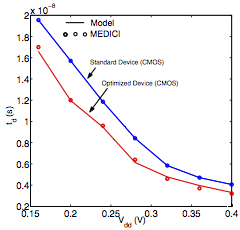
\includegraphics[width=0.4\textwidth]{raychowdhury_doping.png}
    \caption{Effect of sub threshold slope optimization on delay at different voltages.~\cite{Raychowdhury:2006fu}}
    \label{fig:doping}
\end{figure}
 
Although Dreslinski is correct that several research groups have shown optimizations that allow sub-threshold devices to operate at a reduced delay\cite{Dreslinski:2010ez}, citing these as evidence that near-threshold delay can also be improved is misleading. Near-threshold devices, by their very definition, operate in a different region of the transistor's current-voltage curve and optimizations for sub-threshold operation will have a greatly diminished effect on near-threshold delays.